\documentclass[11pt,a4paper]{article}
    \usepackage[margin=2.5cm]{geometry}
    \usepackage{enumitem}
    \usepackage{hyperref}
    \usepackage{tikz}
    \usetikzlibrary{arrows.meta,positioning,shapes.geometric}
    \title{Mathematical Plotting Tools}
    \author{CBBL Tools}
    \date{\today}

    \tikzset{
      methodbox/.style={
        rounded corners=6pt,
        draw=blue!50!black,
        line width=0.9pt,
        fill=blue!6,
        minimum width=13cm,
        text width=11.8cm,
        align=left,
        inner sep=8pt
      }
    }

    \begin{document}
    \maketitle

    \section*{Scope}
    This folder mixes Python notebooks and MATLAB scripts to visualize elementary mathematical objects such as functions, vectors, planes, and Bezier curves.

    \section*{Material in this folder}
    \begin{itemize}[leftmargin=*]
\item \texttt{Functions\_plots.ipynb}
\item \texttt{PlotVectors.ipynb}
\item \texttt{Pla2D.m}
\item \texttt{polinomisBeziers.m}
\item \texttt{polinomisBeziers.mlx}
    \end{itemize}

    \section*{Method summary}
    \begin{itemize}[leftmargin=*]
\item \textbf{Function plotting}. The plotting notebook samples mathematical functions and renders them with standard plotting libraries.
\item \textbf{Vector representation in two and three dimensions}. The vector notebook illustrates geometric operations and coordinate interpretation.
\item \textbf{Bezier polynomial construction}. The MATLAB scripts derive cubic Bezier basis polynomials and use them to trace parametric curves.
\item \textbf{Plane quadrant visualization}. The 2D-plane MATLAB script places random points and annotates the four quadrants of Cartesian space.
    \end{itemize}

    \section*{Method scheme}
    Figure~\ref{fig:summary} is drawn directly in LaTeX with TikZ. It is a compact conceptual map of the main workflows discussed in this folder.

    \begin{figure}[ht]
    \centering
    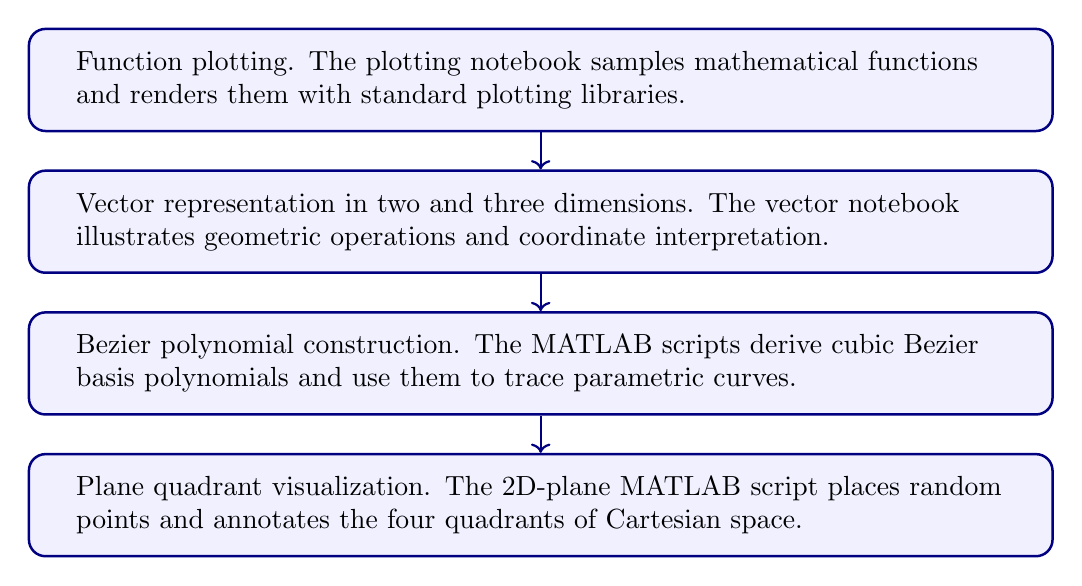
\begin{tikzpicture}[x=1cm,y=1cm]
    \node[methodbox] (m0) at (0,0.0) {Function plotting. The plotting notebook samples mathematical functions and renders them with standard plotting libraries.};
    \node[methodbox] (m1) at (0,-1.8) {Vector representation in two and three dimensions. The vector notebook illustrates geometric operations and coordinate interpretation.};
    \node[methodbox] (m2) at (0,-3.6) {Bezier polynomial construction. The MATLAB scripts derive cubic Bezier basis polynomials and use them to trace parametric curves.};
    \node[methodbox] (m3) at (0,-5.4) {Plane quadrant visualization. The 2D-plane MATLAB script places random points and annotates the four quadrants of Cartesian space.};
    \draw[->, thick, color=blue!50!black] (m0.south) -- (m1.north);
    \draw[->, thick, color=blue!50!black] (m1.south) -- (m2.north);
    \draw[->, thick, color=blue!50!black] (m2.south) -- (m3.north);
    \end{tikzpicture}
    \caption{Conceptual scheme for the methods in the mathTools folder.}
    \label{fig:summary}
    \end{figure}

    \end{document}
